%
%  This simple example illustrates how documents can be
%  split into smaller segments, each segment processed
%  by latex2html separately.  This document can be
%  processed through latex and latex2html with the
%  corresponding makefile.
%

\documentclass{article}         % Must use LaTeX 2e
\usepackage[plainpages=false, colorlinks=true, citecolor=black, filecolor=black, linkcolor=black, urlcolor=black]{hyperref}		
\usepackage[left=.75in,right=.75in,top=.75in,bottom=.75in]{geometry}
\usepackage{makeidx,color,boxedminipage}
\usepackage{graphicx,float}
\usepackage{amsmath,amsthm,amsfonts,amscd,amssymb} 

%%%%%%%%%%%%%%%%%%%%%%%%%%%%%%%%%%%%%%%%%%%%%%%%%%%%%%%%%%%%%%%%%%%%%%
%	Some math support.					     %
%%%%%%%%%%%%%%%%%%%%%%%%%%%%%%%%%%%%%%%%%%%%%%%%%%%%%%%%%%%%%%%%%%%%%%
%
%	Theorem environments (these need the amsthm package)
%
%% \theoremstyle{plain} %% This is the default

\newtheorem{thm}{Theorem}[section]
\newtheorem{cor}[thm]{Corollary}
\newtheorem{lem}[thm]{Lemma}
\newtheorem{prop}[thm]{Proposition}
\newtheorem{ax}{Axiom}

\theoremstyle{definition}
\newtheorem{defn}{Definition}[section]

\theoremstyle{remark}
\newtheorem{rem}{Remark}[section]
\newtheorem*{notation}{Notation}
\newtheorem*{exrcs}{Exercise}
\newtheorem*{exmple}{Example}

%\numberwithin{equation}{section}


%%%%%%%%%%%%%%%%%%%%%%%%%%%%%%%%%%%%%%%%%%%%%%%%%%%%%%%%%%%%%%%%%%%%%%
%	Macros.							     %
%%%%%%%%%%%%%%%%%%%%%%%%%%%%%%%%%%%%%%%%%%%%%%%%%%%%%%%%%%%%%%%%%%%%%%
%
%	Here some macros that are needed in this document:

\newcommand{\motion}{\mathbf{\varphi}}
\newcommand{\hmotion}{\mbox{\boldmath $\hat{\varphi}$}}
\newcommand{\cauchy}{\mbox{\boldmath $\sigma$}}
\newcommand{\eqn}[1]{(\ref{#1})}
\newcommand{\hOmega}{\hat{\Omega}}
\newcommand{\homega}{\hat{\omega}}
\newcommand{\nphalf}{n+\frac{1}{2}}
\newcommand{\nmhalf}{n-\frac{1}{2}}
\newcommand{\kmhalf}{k-\frac{1}{2}}
\newcommand{\kphalf}{k+\frac{1}{2}}
\newcommand{\picdir}{Figures}

\title{PA Recon}
\author{David Fuentes}
\begin{document}                % The start of the document
\maketitle


The presence of deoxyhemoglobin PA signal provides a biomarker for locating
aggressive prostate cancer.  Spectral unmixing to differentiate deoxy- (HHb)
and oxyhemoglobin (HbO2) PA signal is achieved using inverse analysis
applied to physics based models of the reconstruction. 
Modeling the reconstruction involves: (Section~\ref{FluenceSource})
estimating the initial pressure distribution from the absorbed light source
and (Section~\ref{WavePropagation}) propagating the acoustic wave from the
initial pressure distribution to the ultrasound receiver hardware.
An information theoretic mathematical framework for adaptive sampling and 
identifying wavelength and SNR
acquistion parameters that provide the most information content 
with respect to the physics model based data collection
is presented in Section~\ref{GeneralMathFramework}.
The MATLAB script \texttt{exampleRecon.m} documents the user interface
developed, Section~\ref{UserInterface}. 
The interface allows the operator to denote needle insertion
points within the global DICOM frame. GPU kernels are provided
for compute intensive elements of the pipeline to enable high
throughput processing.

%Subtask 2: A likelihood volume will be generated in MATLAB by taking the
%product of all hypoxia maps and corresponding SNR maps and spatially
%registering (based on encoder data) each likelihood map (generated from
%every acquired imaging plane) in a volumetric reference frame.
%
%Subtask 3: A user interface will be developed in MATLAB that allows the
%operator to denote needle insertion points and phantom margins in the global
%reference frame. Although the prototype system detailed herein requires
%offline processing, a future system would permit quasi-real-time
%processing/data registration to allow for iterative (i.e., after each needle
%placement) calculation of the likelihood maps/volume.      
%
%Milestone Achieved: PA-needle imaging data and position data will be
%integrated into a MATLAB-based interface to provide adaptive likelihood
%maps. 

Tradeoffs between accuracy in the physics based predictions and numerical
efficiency are considered within the context of the model-based
reconstruction. A key idea of our approach is that clinically significant
spatial variations of sO2 may be detected using the appropriate numerical
approximations. Ie, full numerical solution to the coupled partial
differential equations that govern the inherent fluence and pressure for
photoacoustic detection are not needed.



%%%%%%%%%%%%%%%%%%%%%%%%%%%%%%%%%%%%%%%%%%%%%%%%%%%%%%%%%%%%%%%%
\section{Mathematical Framework}\label{GeneralMathFramework}
%%%%%%%%%%%%%%%%%%%%%%%%%%%%%%%%%%%%%%%%%%%%%%%%%%%%%%%%%%%%%%%%

The underlying philosophy and assumptions within our approach is that the physics 
models are 1st order accurate or within 70-80\% of the needed accuracy and the error is
adequate within the assumed Gaussian noise.
Gaussian distributions provide analytical representations of the random
variables of interest (ie volume fraction of HHb, $\phi$) within the Bayesian setting and 
provide a crux for understanding. In particular, we say that a random
variable $\eta$ belongs to a multi-variate normal distribution 
of mean $\mu \in \mathbb{R}^n $ and covariance $\Sigma \in \mathbb{R}^{n \times n}$
\[
     \eta \sim \mathcal{N}(\mu,\Sigma)  
    \Rightarrow
      p(\eta)  = \frac{1}{2 \; \pi \; \det{\Sigma}} \exp\left( - \frac{1}{2} \| \mu - \eta\|^2_{\Sigma}\right)
\]


\begin{enumerate}
  \item Our data acquistion model, $\mathcal{G}(\vec{k},\theta): \mathbb{R}^a
\times \mathbb{R}^m \rightarrow \mathbb{R}^n $,
maps deterministic acquisition
parameters, $\vec{k} \in \mathbb{R}^a$, and uncertain parameters, $\theta \in \mathbb{R}^m$
to observables, $\vec{z} \in \mathbb{R}^n$ ( or $\vec{z} \in \mathbb{C}^n$).
Explicitly, we will assume that the
measurement models are corrupted by zero mean white noise noise of a
\textbf{known} covariance matrix, $\Sigma_z \in \mathbb{R}^{n \times n}$ 
\begin{equation}
\label{sensormodelstructure}
\begin{split}
  \vec{z} & = \mathcal{G}(\vec{k};\theta) + \eta   \qquad   \eta \sim \mathcal{N}(0,\Sigma_z)
      \\
  \vec{k} & =  \text{(frequency, laser position, etc)}
      \\
  \theta &  =  \text{(volume fraction, absorption, etc)}
     \end{split}
\end{equation}
$\eta$ may be interpreted as the measurement noise or the acquisition noise
in the sensor model. For a deterministic measurement model $\mathcal{G}$,
the conditional probablity distribution has an explicit analytical form
and may be written as a  \textbf{known} Gaussian
distribution. 
  \[ 
      p(\vec{z}|\theta)   =  \mathcal{N}(\mathcal{G}(\vec{k};\theta),\Sigma_z)  
  \]
  \item Additional \textbf{known} information is the prior probability
distributions for the model parameters, $p(\theta)$.  For simplicity,
    assume that Prior parameters are Gaussian distributed of 
   \textbf{known} mean, $\hat{\theta}$ and covariance, $\Sigma_\theta$
   \[
      \theta \sim \mathcal{N} (\hat{\theta}, \Sigma_\theta)
   \]
  \item Bayes theorem is fundamental to the approach.
The probability of the measurements $p(z)$ must be interprited in terms of the
known information. The probability of the measurements may be derived from
the marginalization of the joint probability and has the interpretation as
the projection of the joint probability onto the measurement axis.
\[
  p(z) = \int_\theta p(\theta,z)  \; d\theta 
       = \int_\theta p(z|\theta) \; p(\theta)\; d\theta 
\]
  \item  The concept of informational entropy~\cite{Madankan15}, $H(Z)$,
provides a mathematically rigorous framework to look for measurement acquisition
parameters, $\vec{k}$, with the high information content of the reconstruction.
Given a probability space 
$(\Omega, \mathcal{F},p)$ (probability maps from the
sigma-algebra of possible events $p:\mathcal{F}\rightarrow [0,1]$
sigma-algebra, $\mathcal{F}$, defined on set of `outcomes' $\Omega$
\cite{durrett2010probability}),
we will define information of an event  as
proportional to the inverse probability.
\[
\text{information} \equiv  \frac{1}{p(z)}
\]
Intuitively, when a low probability event occurs this provides high
information.
The informational entropy is an \textit{average}
of the information content for a sigma algebra of events $\mathcal{F}$
\[
H(Z) = \int_Z  p(z) \ln\frac{1}{p(z)} \; dz
\qquad
  p(z) = \int_\theta p(z|\theta) \; p(\theta)\; d\theta 
\]
Hence this entropy measure is an average of the information content
for a given set of events, $\mathcal{F}$, and is proportional to the
variance or uncertainty in which the set of events occur.
This agrees with thermodynamic entropy;
if the information containing events are completely spread out such as in a
uniform distribution, the entropy is maxmized.
The entropy
is zero for a probability distribution in which
only one event occurs. Zero information is gained when the same event
always occurs ($0 \ln\frac{1}{0} = 0$). 
Intuitively, we want to find acquisition parameters,
$\vec{k}$, for which the measurements are most uncertain
\[
\max_k H(Z)
  \quad \Leftrightarrow \quad
\min_k 
    \int_Z   dz \underbrace{\int_\theta  d\theta \; p(z|\theta) \; p(\theta)}_{p(z)}
                \underbrace{ln \left(\int_\theta  d\theta \; p(z|\theta) \; p(\theta)\right)}_{ln \; p(z)}
\]
Alternatively we may consider this entropy maximization problem as a
sensitivity analysis for the variance of the measurement $Z$, ie . 
$ \max_k H(Z) \approx  \max_k \text{Var}(Z) $
\[ \begin{split}
   \bar{Z} = \mathbb{E}[Z]  & = \int_Z   dz \; z
   \underbrace{\int_\theta  d\theta \; p(z|\theta) \; p(\theta)}_{p(z)}
  \\
   \mathbb{E}[ ( Z - \bar{Z} )^2 ]  & = \int_Z   dz \;(z - \bar{Z})^2 
   \underbrace{\int_\theta  d\theta \; p(z|\theta) \; p(\theta)}_{p(z)}
  \\
   &  \propto
    \int_Z   dz \;(z - \bar{z})^2 \int_\theta  d\theta 
 \exp\left( - \frac{1}{2} \|  z- \mathcal{G}(\vec{k},\theta)  \|^2_{\Sigma_z}\right)
 \exp\left( - \frac{1}{2} \|  \theta - \hat{\theta}  \|^2_{\Sigma_\theta}\right)
 \end{split}
\]
Probilistic integrals may be
computed from uncertainty quantification
techniques~\cite{fahrenholtz2013generalised}.

 

\end{enumerate}


%%%%%%%%%%%%%%%%%%%%%%%%%%%%%%%%%%%%%%%%%%%%%%%%%%%%%%%%%%%%%%%%%%%%%%
\section{Fluence Source}\label{FluenceSource}
%%%%%%%%%%%%%%%%%%%%%%%%%%%%%%%%%%%%%%%%%%%%%%%%%%%%%%%%%%%%%%%%%%%%%%

Reconstruction methods incorporate the spatial distribution of the
absorption and scattering into the expected time dependent photo-acoustic
signal of a single wavelength excitation. 
Diffusion-based light transport
models in turbid media
as well as  directional models of light
propagation using considerations of the delta-Eddington phase function 
are available
\cite{maclellan2013estimating,fuentesetal12a,fuentesetal09,Fuentesetal08}.
A key idea of the inverse analysis is that the optical
absorption provides the image contrast within the spectral unmixing. 
Within our application, the optical absorption, $\mu_a$, is considered a linear
combination of the volume fractions, $\phi$, of deoxy- (HHb) and oxyhemoglobin
(HbO2) constituents.
\[
\mu_a(\lambda,x) = \phi(x) \mu_a^\text{HHb} (\lambda) + (1-\phi(x))\mu_a^\text{HbO2}(\lambda)
\]
Spatial variations in the optical absorption are directly related to hypoxic
regions and will be detected by exploiting the frequency dependence of the
optical properties. Spatial variations in optical parameters are considered
as the spatial decomposition of the prostate domain, $\Omega$
\[
  \Omega = \cup_j \Omega_j
  \qquad \qquad
  \Omega_i \cap \Omega_j = \emptyset  \quad i \neq j
  \qquad \qquad
  \psi_j(x) = 
  \left\{
  \begin{split}
   1 & \quad x    \in \Omega_j \\
   0 & \quad x \notin \Omega_j \\
  \end{split}
   \right.
   \qquad
 \phi(x)  = \sum_{j=1}^{N_\phi} \phi_j \psi_j(x) 
\]

Within the context of our mathematical framework, Section~\ref{GeneralMathFramework},
the volume fraction mixing parameter and the optical parameters are
uncertain model variables, $\theta$. The wavelength is the deterministic
acquisition parameters, $\vec{k}$.
we have little information about the mixing parameter $\phi$ and will
consider this to be uniformly distributed. Optical absorption is both
species and wavelength dependent. We assume that the optical parameters is
Gaussian distributed about the mean of the tabulated spectrum.
\[ 
   \phi_j \sim \mathcal{U}(0,1) 
   \qquad 
  \mu_a^\text{HHb}(\lambda) \sim 
       \mathcal{N}\left( \bar{\mu_a}^\text{HHb}(\lambda) , \Sigma_{\mu_a} \right) 
   \qquad 
  \mu_a^\text{HbO2}(\lambda) \sim 
       \mathcal{N}\left( \bar{\mu_a}^\text{HbO2}(\lambda) , \Sigma_{\mu_a} \right) 
\]
\[
  \theta = 
  \left(
   \phi_1, ... , \phi_{N_\phi},
  \mu_a^\text{HHb}(\lambda) ,
  \mu_a^\text{HbO2}(\lambda)
  \right)
  \qquad \qquad \qquad
   \vec{k} = \lambda
\]

%%%%%%%%%%%%%%%%%%%%%%%%%%%%%%%%%%%%%%%%%%%%%%%%%%%%%%%%%%%%%%%%%%%%%%
\subsection{Standard Diffusion Approximation}
%%%%%%%%%%%%%%%%%%%%%%%%%%%%%%%%%%%%%%%%%%%%%%%%%%%%%%%%%%%%%%%%%%%%%%
The starting point for modeling light transport in tissue is the Boltzman
equation for the radiance, $L(\mathbf{r},\hat{s})$.
\begin{equation}\label{TransportEquation}
\hat{s} \cdot \nabla L(\mathbf{r},\hat{s})
+ \mu_t (\mathbf{r})  L(\mathbf{r},\hat{s})
 = 
\mu_s \int_{4\pi} p(\hat{s},\hat{s}') L(\mathbf{r},\hat{s}) \; d \omega
\qquad
\mu_t = \mu_a + \mu_s
\end{equation}
Here the radiance,  $L(\mathbf{r},\hat{s}) $, represents the radiant power per unit
of solid angle about unit vector $\hat{s}$ and per unit area perpendicular
$\hat{s}$.
The Boltzman equation represents a conservation of energy applied to light
energy transport in tissue at point $r$.
The phase function, $p(\hat{s},\hat{s}')$, provides a measure of the
probability of a scattering photons traveling in direction $\hat{s}'$ 
into the direction $\hat{s}$. The mean cosine  of the scattering angle
is known as the anisotropy factor, $g$
\[
 \int_{4\pi} p(\hat{s} \cdot \hat{s}')(\hat{s} \cdot \hat{s}') d\omega' \equiv g
\]

By convention, the radiance is considered as the summation of a
\textit{known} primary light source with irradiance, $E(\mathbf{r})$, traveling in
direction $s_0$ and scattered light source.
\[
  L(\mathbf{r},\hat{s}) = L_p(\mathbf{r},\hat{s}) + L_s(\mathbf{r},\hat{s})
               = \frac{E(\mathbf{r})  \delta( 1 - \hat{s} \cdot \hat{s}_0)}{
2\pi}  + L_s(\mathbf{r},\hat{s})
\]
The scattered radiance may be represented as sum of spherical harmonics,
this is known as the P-n approximation\cite{Welch95,Modest2003}. 
\[
  L_s(\mathbf{r},\hat{s})  = \sum^\infty_i L_i(\mathbf{r}) P_i(\hat{s})
\]
When only the first two terms are used, this is known as the
P-1\cite{Modest2003} or diffusion approximation\cite{Modest2003}. 
\begin{equation} \label{DiffusionApproximation}
  L_s(\mathbf{r},\hat{s})  \approx \frac{1}{4 \pi} \varphi_d(\mathbf{r}) + \frac{3}{4} \mathbf{j}(\mathbf{r}) \cdot \hat{s}
\end{equation}
When i=0,1,2,3 terms are kept, this is known as the P-3
approximation. The P-2 approximation is generally less accurate and not
used\cite{Modest2003}.

The diffusion model for light transport is valid under the assumption
that light is scattered more than absorbed.
\[
\mu_a << \mu_s(1-g)  \Rightarrow \mu_{eff} << \mu_t
\]

The PDE for the SDA is obtained in two steps by (i) substituting \eqn{DiffusionApproximation}
into \eqn{TransportEquation} and integrating over all solid angles and (ii)
multipling \eqn{TransportEquation}  by $\hat{s}$ and integrating over all
solid angles. Combining the result yeilds
\[ \begin{split}
\nabla\cdot \left( \frac{1}{3 \mu_{tr} } \nabla \varphi_d(\mathbf{r}) \right)  & - \mu_a \varphi_d(\mathbf{r}) 
= 
- \mu_s E(\mathbf{r})
+ \nabla  \cdot  \left( \frac{g \mu_s }{\mu_{tr}} E(\mathbf{r})  \hat{s}_0 \right) 
\\
& \mathbf{j}(\mathbf{r}) = \frac{-1}{3 \mu_{tr}} 
\left[
 \nabla \varphi_d(\mathbf{r}) - 3 g \mu_s E(\mathbf{r}) \hat{s}_0
\right]
\end{split}
\qquad
\begin{split}
\mu_s' = \mu_s (1-g)
\quad
\mu_{tr} = \mu_a + \mu_s'
\\
\mu_{eff} = \sqrt{3\mu_a  \mu_{tr}}
\end{split}
\]
$\mathbf{j}$ is the radiant flux, $\hat{z}$ is the direction of the collimated light, etc...
%%%%%%%%%%%%%%%%%%%%%%%%%%%%%%%%%%%%%%%%%%%%%%%%%%%%%%%%%%%%%%%%%%%%%%
\subsection{Homogenious Coefficients}
%%%%%%%%%%%%%%%%%%%%%%%%%%%%%%%%%%%%%%%%%%%%%%%%%%%%%%%%%%%%%%%%%%%%%%
Through the diffusion model,
the scattered fluence $z$ is obtained from the 
known irradiance $E(x,t)$ (primary source of photons) 
and its flux $\textbf{F}(x,t)$~\cite{fuentesetal10a}.
The total fluence at a point is given by the
sum of the scattered and primary light $\varphi_t(x,t) = z(x,t) + E(x,t)$.
The irradiance is provided by a photon flux emitted throughout
the domain of an interstitial laser fiber $\Omega_{tip}$.
The photons are emittied by an applied power density,
$P^* \left[\frac{W}{m^3}\right]$. Each position in the domain 
$\hat{x} \in \Omega_{tip}$
is treated as a point source of irradiance
\[
dE(x,\hat{x})= 
             \frac{P^*(t)d\hat{x}}{4\pi \|\textbf{x} -
\hat{\textbf{x}}\|^2}
\]
The total irradiance and flux is the integral of each attenuated point source.
\[
\begin{split}
E(x,t) & = \int_{\Omega_{tip}} 
             \frac{P^*(t)}{4\pi \|\textbf{x} - \hat{\textbf{x}}\|^2}
             \exp\left(\mu_t^*(\textbf{x},m)
                         \|\textbf{x} - \hat{\textbf{x}}\|\right) d\hat{x}
 \\
\textbf{F}(x,t) & = \int_{\Omega_{tip}} 
             \frac{P^*(t)}{4\pi \|\textbf{x} - \hat{\textbf{x}}\|^2}
             \exp\left(\mu_t^*(\textbf{x},m) 
                         \|\textbf{x} - \hat{\textbf{x}}\|\right) 
\frac{\textbf{x} - \hat{\textbf{x}} }{ \|\textbf{x} - \hat{\textbf{x}}\| }
d\hat{x}
\end{split} 
\]
\[
  \mu_t^*(\textbf{x},m)  = 
                 \mu_a(\textbf{x},m) + 
                 \mu_s(\textbf{x},m)  
\]
An analytic solution may be obtained by approximating the integral for
the irradiance and flux as
\[
\begin{split}
E(x,t) 
  & \approx 
  \sum_{e\in \Omega_{tip}} E_e(x,t)
  =
  \sum_{e\in \Omega_{tip}} 
          \frac{\Delta V_e P^*(t)}{4\pi \|\textbf{x} - \hat{\textbf{x}}_e\|^2}
          \exp\left(\mu_t^*(\textbf{x},m) 
                 \|\textbf{x} - \hat{\textbf{x}}_e\|\right) 
 \\
\textbf{F}(x,t) 
  & \approx 
    \sum_{e\in \Omega_{tip}} \textbf{F}_e(x,t) 
  = \sum_{e\in \Omega_{tip}} 
          \frac{\Delta V_e P^*(t)}{4\pi \|\textbf{x} - \hat{\textbf{x}}\|^2}
          \exp\left(\mu_t^*(\textbf{x},m) 
                         \|\textbf{x} - \hat{\textbf{x}}\|\right) 
\frac{\textbf{x} - \hat{\textbf{x}} }{ \|\textbf{x} - \hat{\textbf{x}}\| }
\end{split} 
\]
where $\Delta V_e$ is the volume and 
$\hat{\textbf{x}}_e$ is the centroid.
By linearity, each element in the discretization may be treated as
an uncoupled and independent source in the light diffusion equation.
\[
 -{\color{black}\mu_a(\textbf{x})} z_e 
 +{\color{black}\mu_s^*(\textbf{x},m)} E_e
 = \nabla \cdot 
   \left( 
   - \frac{ \nabla z_e }{3\mu_{tr}(\textbf{x},m)} 
   + \frac{ {\color{black}\mu_s^*}(\textbf{x},m) g^* }{3\mu_{tr}(\textbf{x},m)} 
       (\textbf{F})_e
   \right) \qquad \forall e \in \Omega_{tip}
\]
The fluence resulting from each element source $(\varphi_t)_e$
may be obtained from the classical isotropic point source
solution \cite{Welch95}.
The total emanating fluence is the superposition of the element wise
solutions and reduces to a volume weighted sum over the elements.
\[
   \varphi_t = \sum_{e \in \Omega_{tip}}
 {\color{black}P^*(t)}  V_e  \left(
   \frac{3\mu_{tr} \exp(-\mu_{eff} \|\textbf{x} -{\color{black}\textbf{x}_e}\|) }
      {4\pi \|\textbf{x}-{\color{black}\textbf{x}_e}\|}
 - 
      \frac{ 
             \exp(-\mu_t^* \|\textbf{x} -{\color{black}\textbf{x}_e}\|) }
           {2\pi \|\textbf{x}-{\color{black}\textbf{x}_e}\|^2}
   \right)
\approx
    \sum_{e \in \Omega_{tip}}
 {\color{black}P^*(t)}  V_e 
   \frac{3\mu_{tr} \exp(-\mu_{eff} \|\textbf{x} -{\color{black}\textbf{x}_e}\|) }
      {4\pi \|\textbf{x}-{\color{black}\textbf{x}_e}\|}
\]
\[
 \mu_{eff}(\textbf{x},m)  = 
           \sqrt{ 3 {\color{black}\mu_a(\textbf{x},m)} \mu_{tr}(\textbf{x},m) }
\]


%%%%%%%%%%%%%%%%%%%%%%%%%%%%%%%%%%%%%%%%%%%%%%%%%%%%%%%%%%%%%%%%%%%%%%
\section{Wave Propagation}\label{WavePropagation}
%%%%%%%%%%%%%%%%%%%%%%%%%%%%%%%%%%%%%%%%%%%%%%%%%%%%%%%%%%%%%%%%%%%%%%

Computer models of the partial differential equation governing the
propagation of the acoustic wave are expensive. Approximations using k-space
methods and greens function techniques for back projection will be
utilized....

%%%%%%%%%%%%%%%%%%%%%%%%%%%%%%%%%%%%%%%%%%%%%%%%%%%%%%%%%%%%%%%%
\section{User Interface}\label{UserInterface}
%%%%%%%%%%%%%%%%%%%%%%%%%%%%%%%%%%%%%%%%%%%%%%%%%%%%%%%%%%%%%%%%

Example code and user interface is provided from the project site,\\
\texttt{https://github.com/ImageGuidedTherapyLab/PALikelihoodMap}.
GPU kernels use a grid stride loop design pattern for compute intensive
physics model calculations.
The MATLAB script \texttt{exampleRecon.m} computes the wavelength
sensitivity in two steps.
\begin{enumerate}
\item
Uncertainty quantification techniques are applied to compute the variance
of the photoacoustic source,
Section~\ref{GeneralMathFramework} and Section~\ref{FluenceSource}.
\item  Sensitivity statistics are propagated through our photo acoustic
model for the wave propagation, Section~\ref{WavePropagation}.
\end{enumerate}
The SDA fluence model is  proportional to 
photoacoustic source,  $S(r) \left[\frac{W}{m^3}\right]$, 
with a proportionality constant given by the \textit{dimension-less}
Gruneisen parameter, $\Gamma = \frac{v_s^2 \beta}{c_p} $ \\
\fbox{\begin{minipage}{.9\textwidth}
\[
  \text{PA source} =   S(r) = 
  \Gamma  \mu_a \varphi_t  \propto 
 \sum_e
 P^*(t) V_e
   \frac{\mu_{eff}^2 \exp(-\mu_{eff}(\textbf{x})  
         \|\textbf{x} -\textbf{x}_e\|) }
      {4\pi \|\textbf{x}-\textbf{x}_e\|}
\]
\[
  \mu_{eff}  = \sqrt{ 3 {\mu_a} \mu_{tr} }
\quad
 \mu_{tr} = \mu_a  + \mu_s (1-g)
\]
\[
\mu_a(\lambda,x) = \phi(x) \mu_a^\text{HHb} (\lambda) + (1-\phi(x))\mu_a^\text{HbO2}(\lambda)
\]
\end{minipage} }

\begin{figure}[h]
\centering
\begin{tabular}{cc}
\scalebox{0.47}{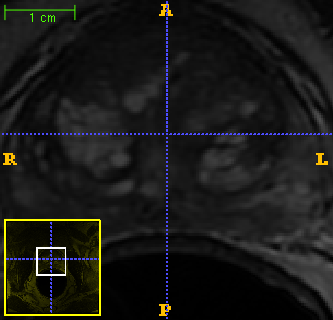
\includegraphics{\picdir/snapshot0002.png}} &
\scalebox{0.47}{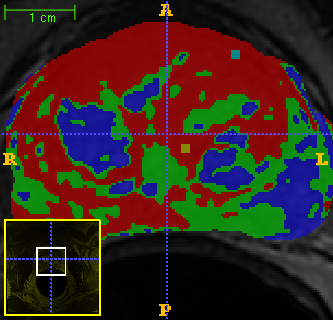
\includegraphics{\picdir/snapshot0001.png}}
\end{tabular}
\[
  \Omega = \cup_j \Omega_j
  \qquad \qquad
  \Omega_i \cap \Omega_j = \emptyset  \quad i \neq j
  \qquad \qquad
  \psi_j(x) = 
  \left\{
  \begin{split}
   1 & \quad x    \in \Omega_j \\
   0 & \quad x \notin \Omega_j \\
  \end{split}
   \right.
   \qquad
 \phi(x)  = \sum_{j=1}^{N_\phi = 3} \phi_j \psi_j(x) 
\]
\caption{
The spatial decomposition is given by a three constituent Gaussian mixture
model applied to pre-procedural imaging.
The label map also encodes the laser applicator location (Label = 4 =
applicator centroid, Label = 5 = entry point).
} \label{SpatialBasis}
\end{figure}
Assuming each parameter is independent, the parameter space probability
function is the tensor product of the individual distributions.
\[
\begin{split}
  \theta & = 
  \left(
   \phi_1, ... , \phi_3,
  \mu_a^\text{HHb}(\lambda) ,
  \mu_a^\text{HbO2}(\lambda)
  \right)
  \\
  \mu_a & = 
  \left(   \theta_1 \psi_1(x) + \theta_2 \psi_2(x) + \theta_3 \psi_3(x)  \right)
     \theta_4
  \\
  & + 
  \left(1- \theta_1 \psi_1(x) + \theta_2 \psi_2(x) + \theta_3 \psi_3(x)  \right)
     \theta_5
\end{split}
 \qquad
  p(s|\theta) =  
       \frac{1}{ \sqrt{2\; \pi \; \Sigma_s}}
       \exp^{-\frac{(s - \Gamma \mu_a \varphi_t )^2}{2 \; \Sigma_s}}
\]
\[
  p(\theta) =  
     \underbrace{1}_{\mathcal{U}(0,1)} \cdot
     \underbrace{1}_{\mathcal{U}(0,1)} \cdot
     \underbrace{1}_{\mathcal{U}(0,1)} \cdot
     \underbrace{
       \frac{1}{ \sqrt{2\; \pi \; \Sigma_{\mu_a}}}
       \exp^{-\frac{(\theta_4 -\bar{\mu_a}^\text{HHb}(\lambda))^2}{2 \; \Sigma_{\mu_a}}}
                }_{ 
       \mathcal{N}\left( \bar{\mu_a}^\text{HHb}(\lambda) , \Sigma_{\mu_a} \right) 
                }
       \cdot
     \underbrace{
       \frac{1}{ \sqrt{2\; \pi \; \Sigma_{\mu_a}}}
       \exp^{-\frac{(\theta_5 -\bar{\mu_a}^\text{HbO2}(\lambda))^2}{2 \; \Sigma_{\mu_a}}}
                }_{ 
       \mathcal{N}\left( \bar{\mu_a}^\text{HbO2}(\lambda) , \Sigma_{\mu_a} \right) 
                }
\]
\begin{table}[h]
\caption{
Constitutive
Data used in numerical
simulations~\cite{welch1984thermal,duck1990}}\label{modelparamaters}
\centering
\begin{tabular}{|c|c|c|c|c|c|c|c|c|c|} \hline
$\bar{\mu_a}^\text{HHb}(750nm) $ $ \frac{1}{ m }$ 
& 
$\bar{\mu_a}^\text{HHb}(850nm) $ $ \frac{1}{ m }$ 
& 
$\bar{\mu_a}^\text{HbO2}(750nm) $ $ \frac{1}{ m }$ 
& 
$\bar{\mu_a}^\text{HbO2}(850nm) $ $ \frac{1}{ m }$ 
& 
 $g$  &
$\mu_s$ $\frac{1}{cm}$  &  $\sqrt{\Sigma_{\mu_a}}$  $\frac{1}{m}$  
 &
$\Gamma$
\\ \hline
          7.e2              &             4.e2            & 5.e2  &
6.e2              &       0.9                  &  140.e2
&            1.e1                      &                  .45          \\
\hline
\end{tabular}
\end{table}

Uncertainty quantification
techniques~\cite{fahrenholtz2013generalised} are used to evaluate sensor
model statistics.
\[ 
   \bar{S}(\lambda)  = \mathbb{E}[S]   = \int_S   ds \; s
   \underbrace{\int_\theta  d\theta \; p(s|\theta) \; p(\theta)}_{p(s)}
  \qquad
   \text{Var}(S)(\lambda)   = 
   \mathbb{E}[ ( S - \bar{S} )^2 ]   = \int_S   ds \;(s - \bar{S})^2 
   \underbrace{\int_\theta  d\theta \; p(s|\theta) \; p(\theta)}_{p(s)}
\]
\[ \begin{split}
 p(s)  &= 
   \int_0^1
   \int_0^1
   \int_0^1
   \int_\mathbb{R}
   \int_\mathbb{R}
                d\theta \; p(s|\theta) \; 
       \frac{1}{ \sqrt{2\; \pi \; \Sigma_{\mu_a}}}
       \exp^{-\frac{(\theta_4 -\bar{\mu_a}^\text{HHb}(\lambda))^2}{2 \; \Sigma_{\mu_a}}}
       \frac{1}{ \sqrt{2\; \pi \; \Sigma_{\mu_a}}}
       \exp^{-\frac{(\theta_5 -\bar{\mu_a}^\text{HbO2}(\lambda))^2}{2 \; \Sigma_{\mu_a}}}
  \\
   & =
   \int_0^1
   \int_0^1
   \int_0^1
   \int_\mathbb{R}
   \int_\mathbb{R}
                d\theta \;
       \frac{1}{ \sqrt{2\; \pi \; \Sigma_s}}
       \exp^{-\frac{(s - \Gamma \mu_a(\theta) \varphi_t(\theta) )^2}{2 \; \Sigma_s}}
             \;
       \frac{1}{ 2\; \pi \; \Sigma_{\mu_a}}
       \exp^{-\frac{(\theta_4 -\bar{\mu_a}^\text{HHb}(\lambda))^2+(\theta_5 -\bar{\mu_a}^\text{HbO2}(\lambda))^2 }{2 \; \Sigma_{\mu_a}}}
\end{split}
\]

\begin{figure}[h]
\centering
\begin{tabular}{ccc}
\scalebox{0.20}{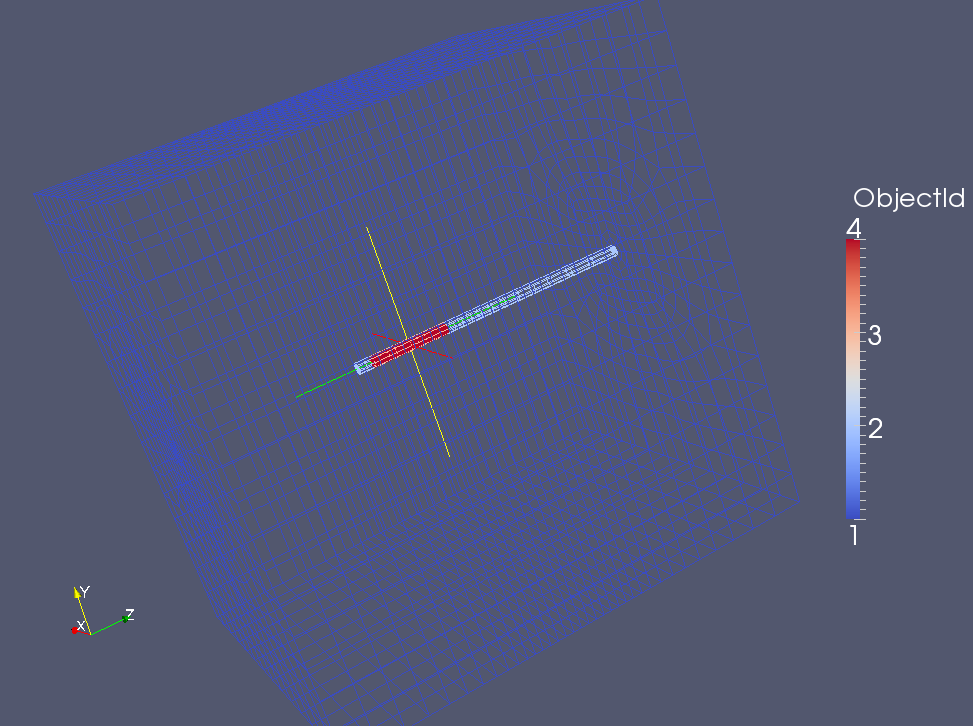
\includegraphics{\picdir/MeshTemplate.png}} &
\scalebox{0.24}{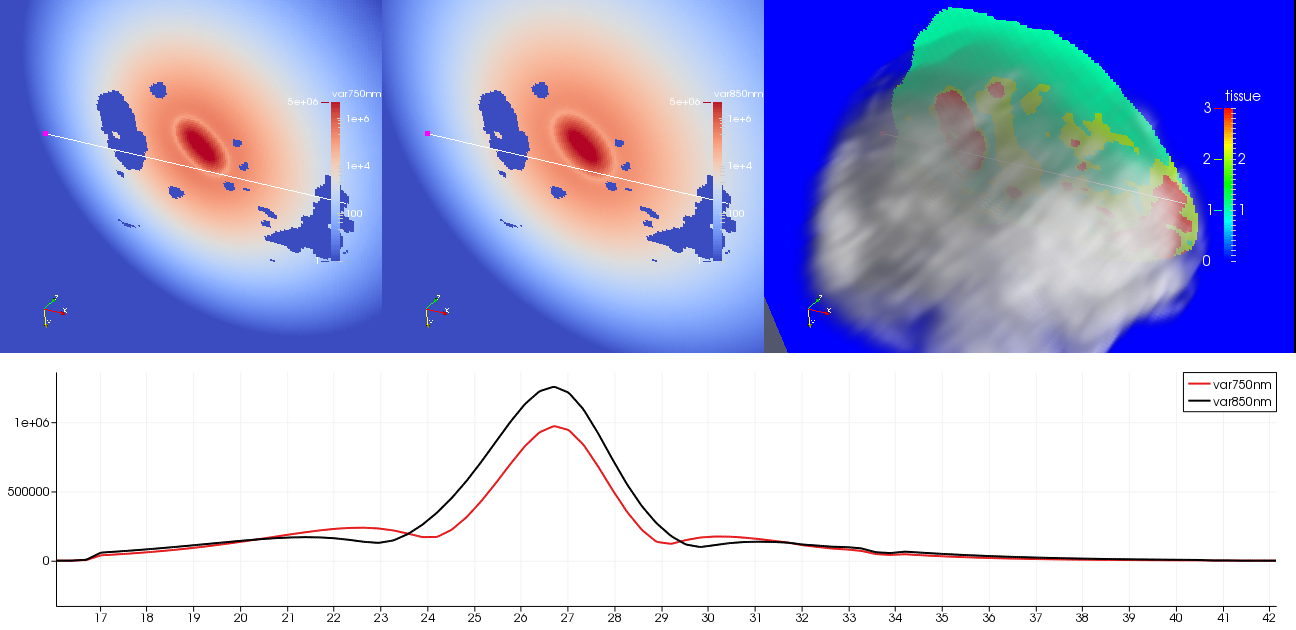
\includegraphics{\picdir/wavelengthsensitivity.png}} \\
(a) & (b)  \\
\end{tabular}
\caption{ Wavelength Sensitivity.
(a) The model of the laser applicator is registered to the prostate
data set shown in Figure~\ref{SpatialBasis}.
(b)
The predicted sensitivity at  $\lambda = 750nm $ and  $\lambda = 850nm $ 
is shown. As expected the photoacoustic source is most sensitive, ie
provides the most information near the laser fiber. Line profiles
quantitatively compare the expected sensitivity with distance from the laser
fiber as well as variations over distinct tissue types.
} \label{DistributionComparison}
\end{figure}

\begin{figure}[h]
\centering
\scalebox{0.47}{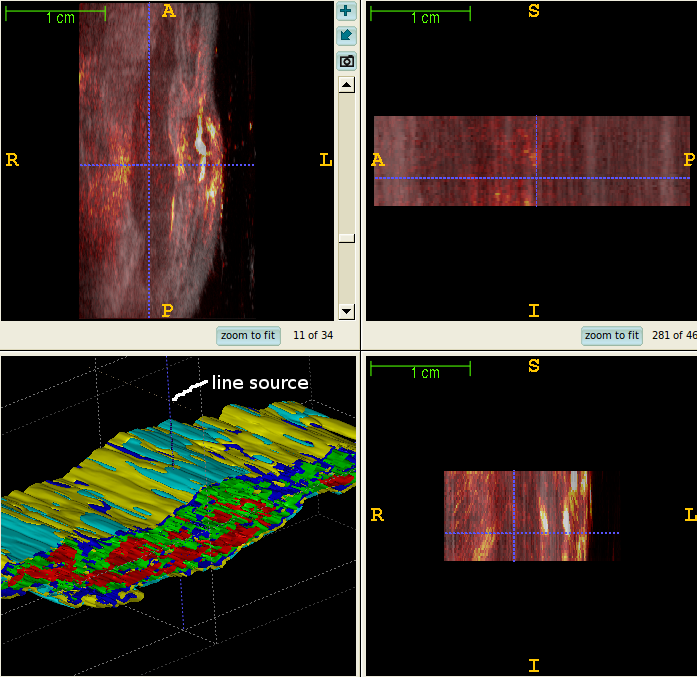
\includegraphics{\picdir/TissuePropertiesLineSource.png}} 
\caption{ Simulation Setup. In this situation. The PA laser source may be
approximated as a photon line source above the tissue surface. }
\end{figure}
%% {
%% \color{blue}
%% Numerical methods for the inverse analysis will include analytical gradient
%% information of the misfit between the predictions of the model based
%% reconstruction against measured data. Gradient information obtained from
%% numerical solutions of the adjoint partial differential equations are known
%% to provide the most efficient numerical solution techniques within a
%% quasi-Newton optimization framework \cite{maclellan2013estimating,fuentesetal12a}. 
%% Alone, model based
%% reconstruction of spatial variations of the optical properties is ill-posed
%% in the sense that not enough information is collected to determine pixel
%% wise variations of the optical properties. Total variation techniques will
%% be applied to regularize the spatial dependence of solution. Additional
%% regularization terms will include prior knowledge of physically acceptable
%% bound of the optical properties. This may also be implemented within a bound
%% constrained optimization framework.
%% All numerical methods will be validated in controlled phantom experiments of
%% known HHb and HbO2 concentrations, see Specific Aim 2. Accurate
%% reconstructions within this controlled setting will provide confidence in
%% applying the numerical techniques in-vivo.
%% }
%%%%%%%%%%%%%%%%%%%%%%%%%%%%%%%%%%%%%%%%%%%%%%%%%%%%%%%%%%%%%%%%
%%%%%%%%%%%%%%%%%%%%%%%%%%%%%%%%%%%%%%%%%%%%%%%%%%%%%%%%%%%%%%%%
\nocite{*}
\bibliographystyle{apalike}
\bibliography{ReconModel}


\end{document}
